\documentclass[12pt]{extarticle}
\usepackage{tempora}
\usepackage[T1, T2A]{fontenc}
\usepackage[utf8]{inputenc}
\usepackage[english, ukrainian]{babel}
\usepackage{geometry}
\usepackage{graphicx}
\usepackage{multirow}
\usepackage{multicol}
\usepackage{float}
\usepackage{indentfirst}
\graphicspath{{/home/artem/Pictures}}
\geometry
{
    a4paper,
    left=30mm,
    top=15mm,
    right=20mm,
    bottom=15mm,
}

\begin{document}
\begin{titlepage}
    \begin{center}
        \textbf{\normalsize{\MakeUppercase{
            Міністерство Освіти і науки України
            Національний університет "Львівська політехніка"
        }}}

        \begin{flushright}
        \textbf{ІКНІ}\\
        Кафедра \textbf{ПЗ}
        \end{flushright}
        \vspace{15mm}

        \includegraphics[width=0.4\textwidth]{lpnu_logo.png}

        \vspace*{\fill}

        \textbf{\normalsize{\MakeUppercase{Звіт}}}
            
        До лабораторної роботи №12

        \textbf{на тему:} “Дослідження роботи DNS сервера та протоколу DHCP.”

        \textbf{з дисципліни:} “Організація комп'ютерних мереж”
            
        \vspace*{\fill}

        \begin{flushright}

            \textbf{Лектор:}\\
            доцент кафедри ПЗ\\
            Крук О.Г.\\
            \vspace{12pt}

            \textbf{Виконав:}\\
            студент групи ПЗ-24\\
            Губик А. С.\\
            \vspace{12pt}

            \textbf{Прийняв:}\\
            доцент кафедри ПЗ\\
            Задорожний І. М.\\
        \vspace{12pt}
        \end{flushright}

        Львів -- 2023
            
            
    \end{center}
\end{titlepage}

\textbf{Тема роботи:} Дослідження роботи DNS сервера та протоколу DHCP.
\vspace{12pt}

\textbf{Мета роботи:} Вивчити принципи роботи DNS, на практиці ознайомитися з принципами роботи
DNS-клієнта на прикладі утиліти nslookup, детально дослідити формат DNS-запиту (і
відповіді) за допомогою Wireshark і nslookup, а також ознайомитися з DHCP-
повідомленнями.
\subsection*{Теоретичні відомості}
Для обміну даними між вузлами мережі використовуються IP-адреси. Однак, людям
простіше запам’ятовувати символьні імена, наприклад, google.com (а не 173.194.39.64) або
somename@gmail.com (а не somename@113.108.11.220). Є і інша причина для застосування
символьних імен: якщо поштовий сервер змінить IP-адресу, символьне ім’я не міняється і
користувачеві не доводиться міняти адресу електронної пошти. Тому, оскільки люди
оперують символьними іменами, а машини – чисельними, то в мережах повинен існувати
якийсь механізм для того, щоб символьним адресам ставити у відповідність IP-адреси (часто
говорять: «відображати символьні імена на IP-адреси»).
На початку розвитку мереж (в мережі ARPAnet, з якої походить Інтернет) цей
механізм був таким. Існував файл hosts.txt, в якому містилася вся інформація про
відповідність всіх символьних імен вузлів і їхніх IP-адрес. Цей файл зберігався на одному
вузлі мережі ARPAnet і в нього при потребі вносилися зміни (наприклад, додавалася
інформація про нові вузли). Інші хости зберігали в себе копії файлу hosts.txt, періодично
завантажуючи поновлену версію hosts.txt зі згаданого «основного» вузла.
З ростом мережі ARPAnet описаний механізм відображення символьних імен в IP-
адреси став неприйнятним з декількох причин. По-перше, очевидно, що з неминучим ростом
мережі файл hosts.txt розрісся б непомірно і синхронізація його «центральної» версії з
копіями на всіх хостах мережі була б проблематичною – є різниця в опрацюванні записів про
кілька сотень і про кілька тисяч вузлів! А по-друге, рано чи пізно трапився б конфлікт імен.
Для розв’язання цих проблем було створено DNS (Domain Name System) – систему
доменних імен. Визначення системи DNS дається у RFC 1034 та 1035.
DNS-система включає в себе три основні компоненти:
У DNS дані про відповідність символьних імен і IP-адрес зберігається у розподілених
базах даних (дані фізично «розкидані» по різних серверах у всьому світі). DNS-сервери
відповідають на запити DNS-клієнтів, шукаючи у базах даних затребувані клієнтами дані про
доменні імена. Ключем пошуку даних є доменне ім’я.
Спрощено схема відображення символьних імен на IP-адреси виглядає так. Нехай
прикладна програма (наприклад, браузер) «знає» символьну адресу і для встановлення TCP-
з'єднання потребує IP-адресу. Ця прикладна програма звертається до бібліотечної процедури,
яка називається «перетворювач IP-адрес» (“resolver”), передаючи символьне ім’я як параметр
цієї процедури. Resolver звертається до DNS-сервера, отримує у відповідь від DNS-сервера
IP-адресу та передає її прикладній програмі.
\break
\subsection*{Хід роботи}

\begin{figure}[H]
    \centering
    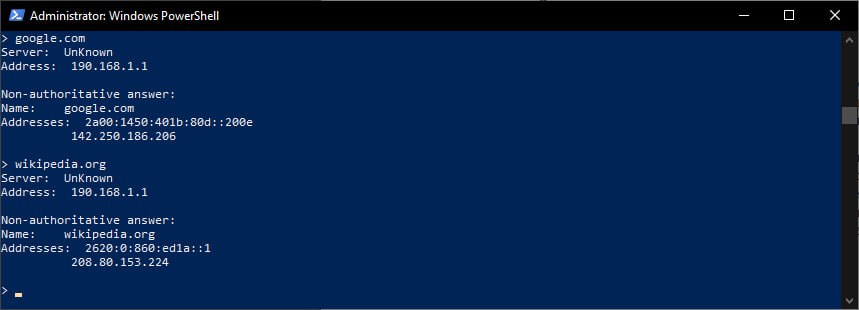
\includegraphics[width=0.90\textwidth]{ip}
    \caption{}
\end{figure}


\begin{figure}[H]
    \centering
    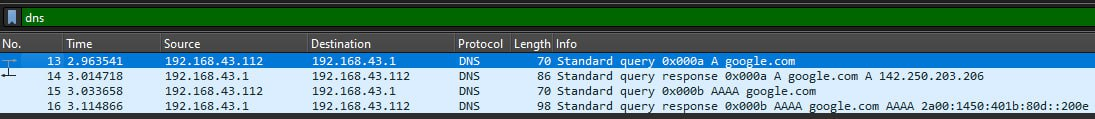
\includegraphics[width=0.90\textwidth]{wireshark}
    \caption{DNS пакети}
\end{figure}

\begin{figure}[H]
    \centering
    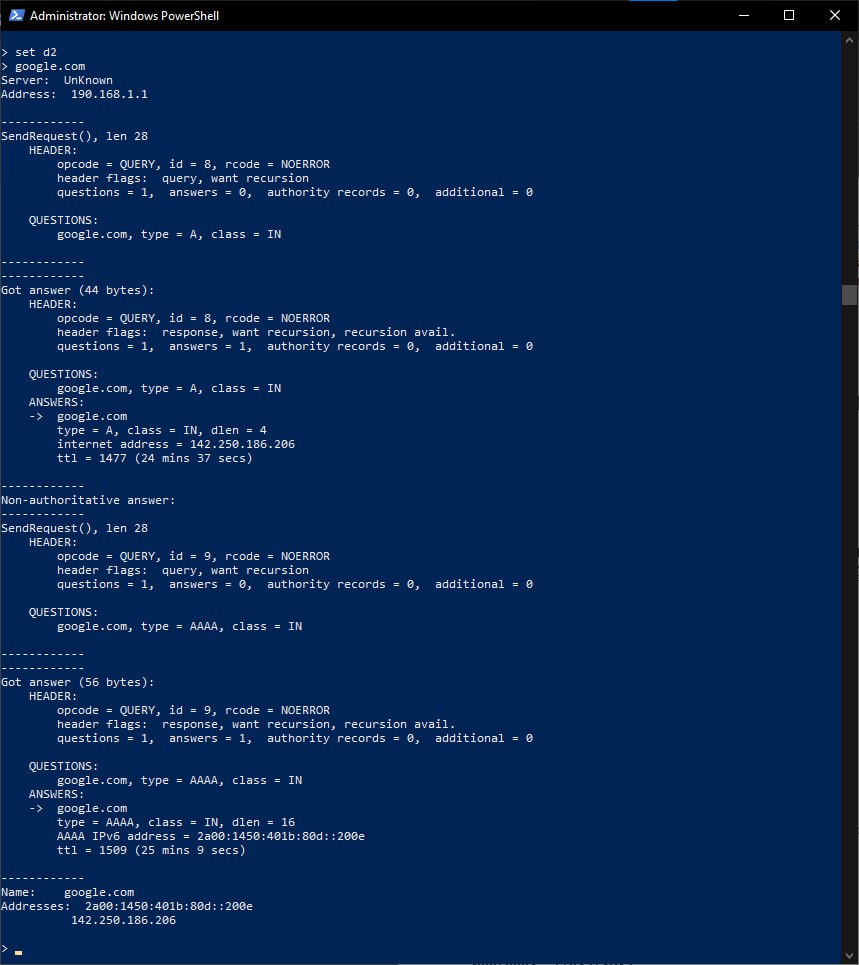
\includegraphics[width=0.90\textwidth]{ipd2}
    \caption{}
\end{figure}

\begin{figure}[H]
    \centering
    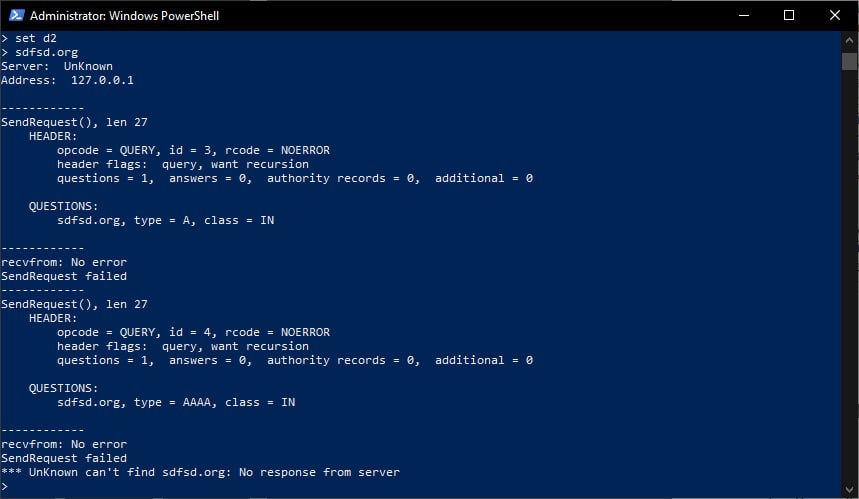
\includegraphics[width=0.90\textwidth]{no_server}
    \caption{}
\end{figure}

\begin{figure}[H]
    \centering
    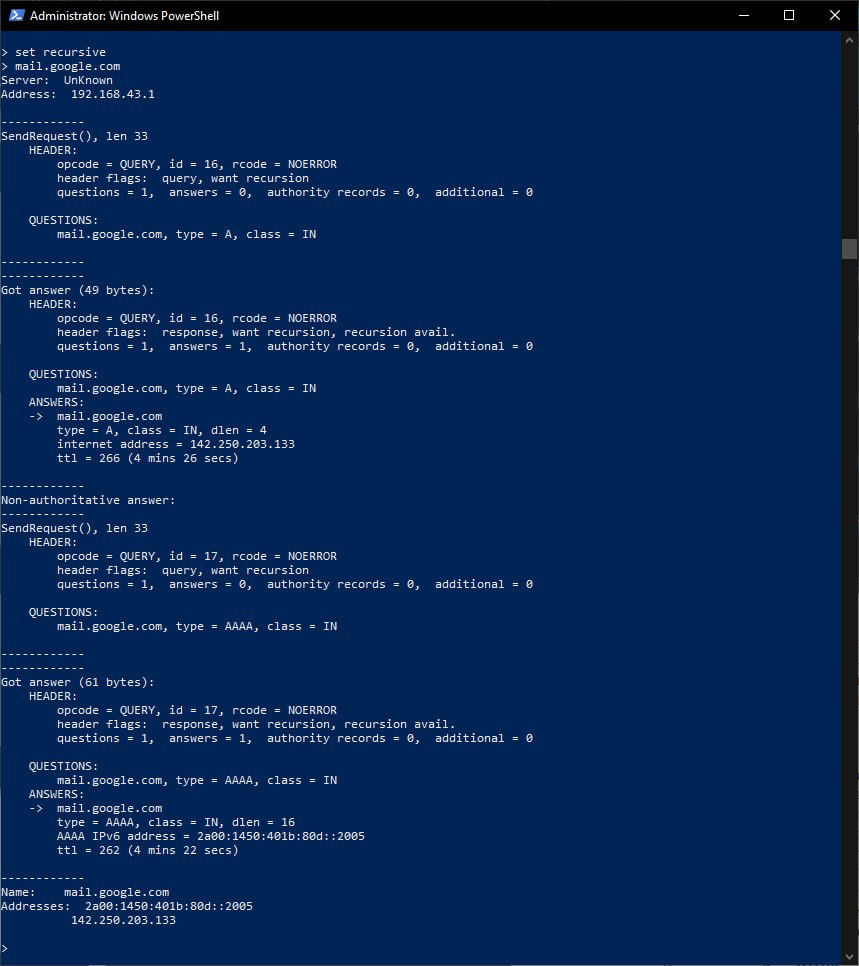
\includegraphics[width=0.90\textwidth]{recursion}
    \caption{}
\end{figure}

\begin{figure}[H]
    \centering
    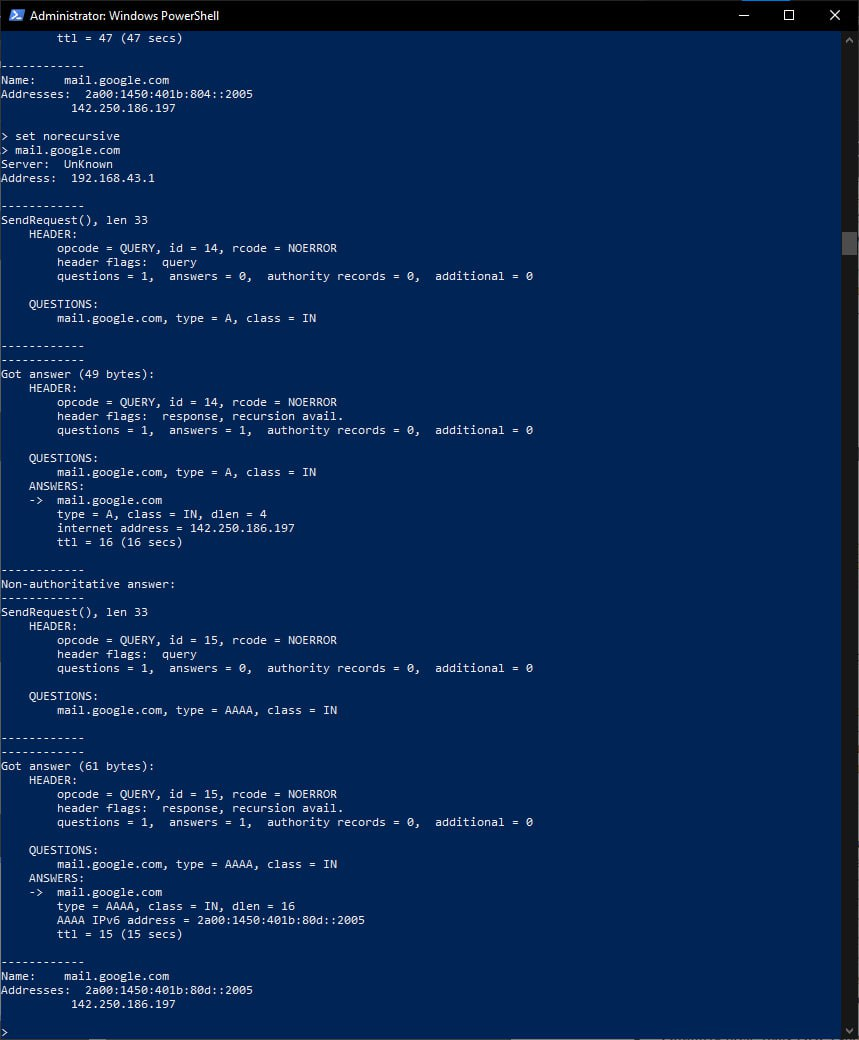
\includegraphics[width=0.90\textwidth]{no_recursion}
    \caption{}
\end{figure}


\begin{figure}[H]
    \centering
    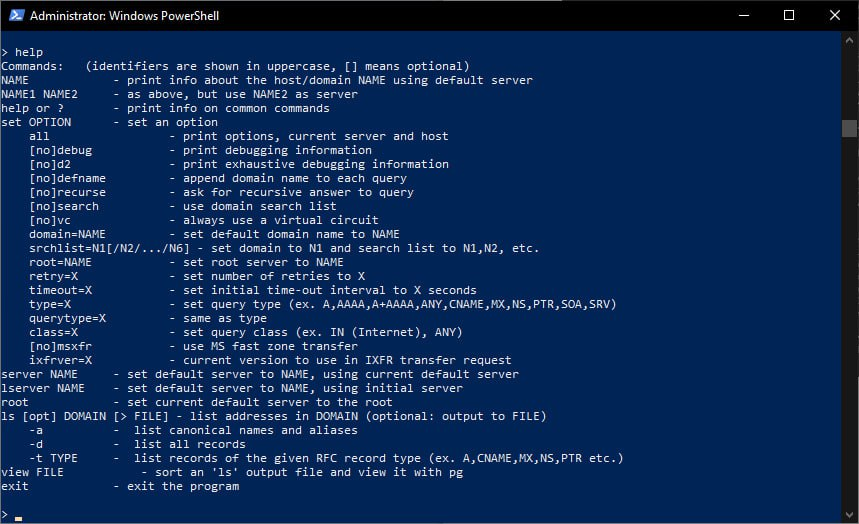
\includegraphics[width=0.90\textwidth]{help}
    \caption{}
\end{figure}

\subsection*{Висновок} 
Я навчився користуватись програмою nslookup і вивчив основні поняття
про DNS сервери.
\end{document}